%\begin{region}
%% ****** Start of file apstemplate.tex ****** %
%%
%%
%%   This file is part of the APS files in the REVTeX 4.2 distribution.%%
%%   Copyright (c) 2024 The American Physical Society.
%%
%%   See the REVTeX 4 README file for restrictions and more information.
%%
%
% This is a template for producing manuscripts for use with REVTEX 4.2
% Copy this file to another name and then work on that file.
% That way, you always have this original template file to use.
%
% Group addresses by affiliation; use superscriptaddress for long
% author lists, or if there are many overlapping affiliations.
%  N.B. The groupedaddress option will reorder the author list based
%  on the order in which affiliations appear. Please be sure to check the author 
%  order. You can also use the unsortedaddress(?) option instead to prevent that
%  behavior.
% For Phys. Rev. appearance, change preprint to twocolumn.
% Choose physrev, prl, or rmp for journal
%  N.B. physrev is appropriate for all APS journals except prl and rmp
%  Add 'draft' option to mark overfull boxes with black boxes
%  Add 'showkeys' option to make keywords appear
\documentclass[aps,physrev,twocolumn,superscriptaddress]{revtex4-2}
%\documentclass[aps,physrev,preprint,superscriptaddress]{revtex4-2}
%\documentclass[aps,prl,preprint,superscriptaddress]{revtex4-2}
%\documentclass[aps,prl,reprint,groupedaddress]{revtex4-2}
%\documentclass[aps,rmp,preprint,superscriptaddress]{revtex4-2}
%\documentclass[aps,rmp,reprint,groupedaddress]{revtex4-2}

% You should use BibTeX and apsrev.bst for references
% Choosing a journal automatically selects the correct APS
% BibTeX style file (bst file), so only uncomment the line
% below if necessary.
%\bibliographystyle{apsrev4-2}


\usepackage{algorithm}
\usepackage{graphicx}
\usepackage{amsmath,amssymb}
\usepackage{braket}
\usepackage{quantikz}

\DeclareMathOperator{\Tr}{Tr}
\DeclareMathOperator{\Enc}{Enc}
\DeclareMathOperator{\Dec}{Dec}

%\end{region}

\begin{document}
%\begin{region}
% Use the \preprint command to place your local institutional report
% number in the upper righthand corner of the title page in preprint mode.
% Multiple \preprint commands are allowed.
% Use the 'preprintnumbers' class option to override journal defaults
% to display numbers if necessary
%\preprint{}

%Title of paper
\title{Noisy Quantum Broadcasting}

% repeat the \author .. \affiliation  etc. as needed
% \email, \thanks, \homepage, \altaffiliation all apply to the current
% author. Explanatory text should go in the []'s, actual e-mail
% address or url should go in the {}'s for \email and \homepage.
% Please use the appropriate macro foreach each type of information

% \affiliation command applies to all authors since the last
% \affiliation command. The \affiliation command should follow the
% other information
% \affiliation can be followed by \email, \homepage, \thanks as well.
\author{Matthew Prest}
\email[]{mprest@gradcenter.cuny.edu}
%\homepage[]{Your web page}
%\thanks{}
\affiliation{Graduate Center of the City University of New York, 365 Fifth Avenue, New York, NY 10016, USA}
\affiliation{Department of Physics and Astronomy, Hunter College of the City
University of New York, 695 Park Avenue, New York, NY 10065, USA}

\author{Author 2}
% \email[]{}
%\homepage[]{Your web page}
%\thanks{}
% \affiliation{Graduate Center of the City University of New York, 365 Fifth Avenue, New York, NY 10016, USA}


%Collaboration name if desired (requires use of superscriptaddress
%option in \documentclass). \noaffiliation is required (may also be
%used with the \author command).
%\collaboration can be followed by \email, \homepage, \thanks as well.
%\collaboration{}
%\noaffiliation

\date{\today}

\begin{abstract}
Quantum networks for the purposes of distributed computing and cryptography rely on transmitting quantum states subject to fundamental constraints such as the no-cloning and no-broadcasting theorems. The use of shared entanglement presents additional utility for quantum networking protocols. In this work, we present a systematic study of the operational robustness and scalability of entanglement-assisted restricted quantum broadcasting, including the conditions under which block-level QEC improves receiver fidelity and the extent to which real-device correlated errors invalidate independent-channel predictions. We analyze a modified quantum broadcasting protocol through numerical simulations, analytical techniques, approximate methods, and real hardware results through IBM's QisKit service. Our results demonstrate significant experimental constraints on the scaling of this broadcasting protocol's effectiveness on current hardware. We show the limitations of quantum error correction in the noisy-intermediate-scale-quantum (NISQ) paradigm. Unusual, quasi-periodic time dependent fidelity features are demonstrated, and we discuss the necessary improvements, both theoretical and experimental in order to achieve practical and scalable quantum broadcasting.
\end{abstract}

% insert suggested keywords - APS authors don't need to do this
%\keywords{}

%\maketitle must follow title, authors, abstract, and keywords
\maketitle
%\end{region}

\section{Introduction \label{Introduction}}
%\begin{region}
Pioneering work in quantum information produced famous impossibility results such as the no-cloning theorem \cite{wootters2009no} and the no-broadcasting theorem \cite{barnum2007generalized}. These results have been fundamental in shaping our understanding of the limitations quantum information and have had profound implications for quantum communication and cryptography \cite{vsupic2020self}. However, recent research has shown that these impossibility results can be circumvented under certain, more restrictive, conditions, leading to new possibilities for quantum information processing \cite{larasati2025towards,zhang2025efficient,sukeno2025quantum,andronikos2023one}. In this paper, we explore the concept of restricted broadcasting, where a quantum state can be broadcast to multiple receivers under specific constraints using shared prior entanglement \cite{PhysRevA.105.042611}.
\\

Broadcasting channels are a key resource in many classical networking protocols~\cite{chang1984reliable}. The inclusion of some form of broadcasting to quantum network protocols has the potential to facilitate new and more efficient functionality. Although current quantum hardware are typically remote quantum servers that are cloud accessible through classical information channels, there is growing interest and experimental realizations of quantum networks, capable of distributing entanglement over hundreds of kilometers~\cite{simon2017towards, pompili2021realization, neumann2022continuous}. Real world quantum networks must navigate the impact of channel noise on transmitted quantum states, this is commonly achieved through a variety of quantum error correction (QEC) schemes \cite{gottesman1997stabilizer}.
\\

We begin with the M-sender N-receiver broadcasting protocol introduced in \cite{sukeno2023broadcasting}, where parties share an initial entangled state from which single qubits are distributed to the receivers. The senders then apply local unitaries to their systems, which add a phase on the receivers' qubits. By measuring in a Fourier basis and broadcasting the classical outcomes, the receivers can apply byproduct corrections to recover the desired state without revealing the sender's choice of phase. This protocol demonstrates that, under certain conditions, it is possible to achieve a form of broadcasting that is not prohibited by the no-broadcasting theorem.
\\

In this work, we extend the M-sender N-receiver broadcasting protocol to account for noisy distribution channels to each receiver. We analyze the impact of noise on the protocol's performance and explore how quantum error correction can be integrated to mitigate the effects of noise \cite{knill1997theory}. By encoding the receivers' qubits using a quantum error-correcting code, we can protect the transmitted information from errors introduced by the noisy channels, thereby enhancing the robustness of the broadcasting protocol. We then implement the noisy broadcasting protocol using numerical simulations where we compare exact and approximate methods, and finally on quantum hardware through IBM's QisKit platform.
%\end{region}

\section{Broadcasting Protocol}
%\begin{region}
We first review the M-sender N-receiver broadcasting protocol from \cite{sukeno2023broadcasting} in the ideal, noiseless case. The protocol involves a resource state shared between the senders and receivers, local private unitaries applied by the senders to add phases, and measurements in a Fourier basis to enable byproduct corrections at the receivers. The protocol uses a classical broadcasting channel to send correction information from the senders to the receivers, but does not require any quantum communication after the initial resource state distribution. Additionally, correction steps do not require revealing the sender's choice of phase, which can be delayed until after the resource state is distributed, preserving a level of privacy in the communication.
\\
For this protocol, the $M$ senders (Alices) possess an $N+1$-dimensional qudit each, while the $N$ receivers possess a single qubit each. The initial resource state is an entangled superposition of symmetric states, where each sender's system is in a state corresponding to the number of receivers in the $\ket{0}$ or $\ket{1}$ state. This is given by
\begin{align}
\ket{\Psi^{(M,N)}}
&:= \sum_{k=0}^{N}\alpha^k\beta^{N-k}\binom{N}{k}^{1/2}
\left(\prod_{j=1}^{M}\ket{k}_{a_j}\right)\ket{k;N-k},
\end{align}
where $\ket{k;N-k}$ is the symmetric state of $N$ qubits with $k$ in the $\ket{0}$ state and $N-k$ in the $\ket{1}$ state.
\\
Each sender $j$ applies a local unitary $U_{a_j}(\theta_j)$ that adds a phase $\theta_j$ depending on the number of $\ket{0}$ and $\ket{1}$ states in the receivers' systems. This is defined as
\begin{align}
U_{a_j}(\theta_j)\ket{k}_{a_j}
&:= e^{i(2k-N)\theta_j}\ket{k}_{a_j},
\qquad \theta_j\in[0, 2\pi].
\end{align}
After the senders apply their unitaries, they measure their systems in the Fourier basis $\{\ket{u_n}\}_{n=0}^N$, where
\begin{align}
\ket{u_n}
&:= \frac{1}{\sqrt{N+1}}\sum_{k=0}^{N} e^{2\pi i nk/(N+1)}\ket{k},
\qquad n\in\{0,1,\dots,N\}.
\end{align}
The measurement outcomes of all senders $\Vec{n}=(n_1,\dots,n_M)$ are then broadcast to the receivers, who apply byproduct corrections $U_{\Vec{n}}$ to their qubits to recover the desired state. The byproduct correction is defined as
\begin{align}
U_{\Vec{n}}\ket{0}
&:= \exp\!\left(\frac{2\pi i}{N+1}\sum_{j=1}^{M}n_j\right)\ket{0},
\\
U_{\Vec{n}}\ket{1}
&:= \ket{1}.
\end{align}
In the ideal, noiseless case, this protocol allows the receivers to recover the state
\begin{align}
\ket{\psi_{\mathrm{target}}}
&= \alpha\,e^{i\sum_{j=1}^{M}\theta_j}\ket{0} + \beta\,e^{-i\sum_{j=1}^{M}\theta_j}\ket{1}.
\end{align}
\\
%
To measure the success of an instance of the protocol we compute the fidelity of the output state with respect to the target state which in general is defined as
\begin{align}
    F(\rho_1, \rho_2) = \big(\Tr\sqrt{\sqrt{\rho_1}\rho_2\sqrt{\rho_1}} \big)^2.
\end{align}
Where $\rho_1, \rho_2$ are the density matrices of the output and target state. For pure states this reduces to 
\begin{align}
    F(\ket{\psi_{\mathrm{out}}}, \ket{\psi_{\mathrm{target}}}) = \mid 
    \braket{\psi_{\mathrm{out}} \mid \psi_{\mathrm{target}}}\mid^2,
\end{align}
and for a circuit with a fixed measurement basis, this can be estimated by appending an additional final unitary that maps the target state to an eigenstate of the measurement basis (e.g. $\ket{0}$), measuring and repeating. 

The senders' $(N{+}1)$-dimensional qudit can be embeded into
\begin{align}
n_q = \lceil \log_2(N+1) \rceil
\end{align}
qubits using a binary encoding: the computational basis state $\ket{k}_{a_j}$ ($0\le k\le N$) is stored as the $n_q$-bit binary representation of $k$. This allows for direct implementation on qubit-based hardware.

%\end{region}

\section{Noisy Channels}
%\begin{region}

In a realistic scenario, the distribution of qubits to the receivers may be subject to noise~\cite{schumacher1996sending, bergou2013introduction}. We model this noise using a depolarizing channel, which acts independently on each qubit sent to the receivers~\cite{dur2005standard}. This is applied after the initial resource state is prepared but before each sender applies their local unitary. The depolarizing channel with depolarizing probability $p$ is defined as
\begin{align}
\mathcal{D}_p(\rho)
&:= (1-p)\rho + \frac{p}{3}\left(X\rho X + Y\rho Y + Z\rho Z\right), \\
&\qquad 0\le p\le 1, \nonumber
\end{align}
where $X$, $Y$, and $Z$ are the Pauli operators. The presence of noise can degrade the fidelity of the output state at the receivers, making it crucial to analyze the performance of the protocol under these conditions and to explore methods for improving the protocol's resilience such as QEC.
%
We illustrate the effects of depolarizing noise through an example with a single sender (Alice) $M=1$ and two identical receivers (Bobs) $N=2$, with a shared resource state given by $\alpha=\beta=1/\sqrt{2}$ and sender angle $\theta$. Specializing Eq.~(1) to these parameters and using the convention that $\ket{k;N{-}k}$ is the symmetric state with $k$ qubits in $\ket{0}$ and $N{-}k$ in $\ket{1}$, the resource state reads
\begin{align}
    \ket{\Psi_{\text{init}}} = \frac{1}{2}\big[&\ket{0}_A\ket{11}_{B} + \ket{1}_A(\ket{01}_{B} + \ket{10}_{B}) + \ket{2}_A\ket{00}_{B}\big].
\end{align}
Here, the labels $A,B$ indicate who is in possession of which qubit; these will be omitted going forward, but the structure remains the same. The target state at each receiver is the equatorial state 
\begin{align}
    \ket{\psi_{\mathrm{target}}} = \frac{1}{\sqrt{2}}\!\left(e^{i\theta}\ket{0} + e^{-i\theta}\ket{1}\right).
\end{align}

We then take the resource-state density matrix $\rho_{\text{init}} = \ket{\Psi_{\text{init}}}\bra{\Psi_{\text{init}}}$ and apply independent depolarizing channels $\mathcal{D}_p$ with $p_1 = p_2 = p$ to each receiver qubit. On the Pauli basis the channel acts as $\mathcal{D}_p(I)=I$ and $\mathcal{D}_p(P)=\eta\,P$ for $P\in\{X,Y,Z\}$, where
\begin{align}
    \eta = 1 - \tfrac{4p}{3}
\end{align}
is the single-qubit Bloch-vector contraction factor. Tracing out Alice's qutrit, the joint receiver density matrix after noise is
\begin{align}
    \rho_{\text{noisy}} &= \tfrac{1}{4}\, I\!\otimes\!I + \tfrac{\eta^2}{8}\big(X\!\otimes\!X + Y\!\otimes\!Y\big),
\end{align}
which, in the basis $\{\ket{00},\ket{01},\ket{10},\ket{11}\}$, takes the matrix form
\begin{align}
    \rho_{\text{noisy}} = \frac{1}{4}\begin{bmatrix}
    1 & 0 & 0 & 0 \\
    0 & 1 & \eta^2 & 0 \\
    0 & \eta^2 & 1 & 0 \\
    0 & 0 & 0 & 1
    \end{bmatrix}.
\end{align}
The single-receiver marginal $\Tr_2[\rho_{\text{noisy}}] = I/2$ remains maximally mixed: the broadcast information is stored in the sender--receiver correlations rather than in the receivers' local states, and only the inter-receiver coherence ($X\!\otimes\!X + Y\!\otimes\!Y$) is suppressed (by $\eta^2$) at this stage.

Alice then applies her phase gate $U_A(\theta)$ to her qutrit, which from Eq.~(2) with $N=2$ is the diagonal unitary
\begin{align}
    U_A(\theta) = \begin{bmatrix}
        e^{-2i\theta} & 0 & 0 \\
        0 & 1 & 0 \\
        0 & 0 & e^{2i\theta}
        \end{bmatrix}.
\end{align}
She then measures her qutrit in the Fourier basis with measurement operators $M_n = \ket{u_n}\bra{u_n}$, where $\ket{u_n} = \frac{1}{\sqrt{3}}\sum_{k=0}^2 e^{2\pi i nk/3}\ket{k}$ for $n=0,1,2$, and broadcasts the outcome $n$ so that each receiver can apply the byproduct correction $U_n = \mathrm{diag}(e^{2\pi i n/3},\,1)$.

Because the depolarizing channels act only on the receivers, they commute with the sender phase gate $U_A$ and the Fourier projector $M_n$, which act only on Alice's qutrit. The byproduct correction $U_n$ also commutes with $\mathcal{D}_p$ since it is diagonal in the computational basis (and so leaves the depolarizing channel covariant on each receiver). As a consequence, each outcome $n\in\{0,1,2\}$ still occurs with probability $P(n)=1/3$ independently of $p$ and $\theta$, and the noisy joint receiver state after measurement and correction can be written as the noise applied to the noiseless output,
\begin{align}
    \rho^{\text{joint}}_{\text{post}} = (\mathcal{D}_p \otimes \mathcal{D}_p)\!\left(\ket{\Psi_{\text{target}}}\!\bra{\Psi_{\text{target}}}\right),
\end{align}
where $\ket{\Psi_{\text{target}}} = \tfrac{1}{2}\big[e^{2i\theta}\ket{00} + (\ket{01}+\ket{10}) + e^{-2i\theta}\ket{11}\big]$ is the noiseless joint output. Tracing out the second receiver gives the single-receiver post-measurement state
\begin{align}
    \rho_{\text{post}} = \mathcal{D}_p\!\big(\ket{\psi_{\mathrm{target}}}\!\bra{\psi_{\mathrm{target}}}\big)
    = \frac{1}{2}\begin{bmatrix} 1 & \eta\, e^{2i\theta} \\ \eta\, e^{-2i\theta} & 1 \end{bmatrix},
\end{align}
i.e.\ the target single-qubit state with its Bloch vector contracted by $\eta=1-4p/3$.

The fidelity with the target state is then
\begin{align}
    F &= \bra{\psi_{\mathrm{target}}}\rho_{\text{post}}\ket{\psi_{\mathrm{target}}} \nonumber \\
    &= \tfrac{1}{2}(1 + \eta) = 1 - \tfrac{2p}{3},
\end{align}
which is independent of the sender angle $\theta$ and reproduces the depolarizing-channel fidelity bound used later in Sec.~IV. The $\theta$-independence follows from the fact that $\mathcal{D}_p$ contracts the Bloch vector isotropically, so every equatorial target state is degraded by the same amount.

%\end{region}

\section{QEC Enhanced Protocol}
%\begin{region}
There are many possible ways to incorporate error correction into the protocol. We choose to encode each receiver's qubit using the $[[5,1,3]]$ maximally efficient single-qubit error code~\cite{laflamme1996perfect,knill1997theory}. This code is defined by its stabilizer generators and logical basis states \cite{gottesman1997stabilizer,calderbank1998quantum}, and it allows us to protect the transmitted information from errors introduced by the depolarizing channels \cite{devitt2013qec}. The encoding and decoding processes involve applying specific unitaries to map between the logical qubits and the physical qubits, as well as performing syndrome measurements to identify and correct errors. By integrating this error correction scheme into the broadcasting protocol, we can enhance the robustness of the communication and improve the fidelity of the output states at the receivers in the presence of noise.

Let $X,Y,Z$ be the single-qubit Pauli operators and $I$ the identity.
On each 5-qubit block, we define stabilizer generators
\begin{align}
g_1 &:= XZZXI, g_2 := IXZZX, \nonumber \\
g_3 &:= XIXZZ, g_4 := ZXIXZ.
\end{align}
From this we define the codespace
\begin{align}
\mathcal{C}
&:= \left\{\ket{\varphi}\in(\mathbb{C}^2)^{\otimes 5} ~:~ g_r\ket{\varphi}=\ket{\varphi}\ \ \forall r\in\{1,2,3,4\}\right\}.
\end{align}
The concrete logical basis we then use that spans $\mathcal{C}$ is
\begin{align}
\ket{0_L} = \frac{1}{4}\big(&\ket{00000}+\ket{10010}+\ket{01001}+\ket{10100} \nonumber \\
+&\ket{01010} -\ket{11011}-\ket{00110}-\ket{11000} \nonumber \\
-&\ket{11101}-\ket{00011}-\ket{11110}-\ket{01111} \nonumber \\
-&\ket{10001} -\ket{01100}-\ket{10111}+\ket{00101}\big),
\\
\ket{1_L}
&:= X^{\otimes 5}\ket{0_L}.
\end{align}
We define the encoding isometry $\Enc:\mathbb{C}^2\to(\mathbb{C}^2)^{\otimes 5}$ by linear extension of
\begin{align}
\Enc(\ket{0}) &:= \ket{0_L}, &
\Enc(\ket{1}) &:= \ket{1_L}.
\end{align}
Then we fix any 5-qubit unitary $V_{\Enc}$ such that, for all $\ket{\psi}\in\mathbb{C}^2$,
\begin{align}
V_{\Enc}\big(\ket{\psi}\otimes\ket{0}^{\otimes 4}\big)
&= \Enc(\ket{\psi}).
\end{align}
We next define the decoding channel $\Dec:(\mathbb{C}^2)^{\otimes 5}\to\mathbb{C}^2$ by
\begin{align}
\Dec(\rho)
&:= \operatorname{Tr}_{2,3,4,5}\!\left[V_{\Enc}^\dagger\,\rho\,V_{\Enc}\right],
\end{align}
where $\operatorname{Tr}_{2,3,4,5}$ traces out the last four qubits of the block.

Using our enlarged state space we can introduce syndrome measurements and correction operators. Given a 5-qubit block state $\rho$, first measure each $g_r$ to obtain eigenvalues $\lambda_r\in\{+1,-1\}$ and define
syndrome bits $s_r\in\{0,1\}$ by $\lambda_r=(-1)^{s_r}$, forming $s=(s_1,s_2,s_3,s_4)\in\{0,1\}^4$. We choose a syndrome-to-correction map $s\mapsto E_s$ into 5-qubit Pauli operators such that
\begin{align}
E_s g_r
&= (-1)^{s_r}\, g_r E_s,
\qquad r\in\{1,2,3,4\},
\end{align}
and (for single-qubit errors) $E_{s(P)}:=P$ for each weight-1 Pauli $P\in\{X_i,Y_i,Z_i\}_{i=1}^5$ with syndrome $s(P)$. Lastly we apply the correction $E_s^\dagger=E_s$ before decoding using the decoding channel.

\subsection{Protocol: $M$-sender $\to$ $N$-receiver broadcasting with $[[5,1,3]]$ quantum error correction over depolarizing channels.}


Fix integers $M\ge 1$ and $N\ge 1$. Let $\alpha,\beta\in\mathbb{C}$ satisfy $|\alpha|^2+|\beta|^2=1$. For each sender $j\in\{1,\dots,M\}$, let $a_j$ be a $(N{+}1)$-dimensional Hilbert space with computational basis $\{\ket{k}_{a_j}\}_{k=0}^N$.For each receiver $\ell\in\{1,\dots,N\}$, let $q_\ell$ be a qubit Hilbert space with computational basis $\{\ket{0}_\ell,\ket{1}_\ell\}$.
    
\begin{enumerate}
    \item \textbf{Prepare resource.} Prepare $\ket{\Psi^{(M,N)}}$ on $(a_1,\dots,a_M,q_1,\dots,q_N)$.
    
    \item \textbf{Encode receivers.} For each $\ell\in\{1,\dots,N\}$, replace $q_\ell$ by a 5-qubit block
    $(b_{\ell,1},\dots,b_{\ell,5})$ by applying $\Enc$:
    \begin{align}
    \ket{\widetilde{\Psi}^{(M,N)}}
    &:= \left(I_{a_1\cdots a_M}\otimes \Enc^{\otimes N}\right)\ket{\Psi^{(M,N)}}.
    \end{align}
    
    \item \textbf{Transmit over noisy channels.} Send each $b_{\ell,t}$ through $\mathcal{D}_p$, independently for all $\ell$ and $t$.
    
    \item \textbf{Sender phase imprinting.} Each sender $j$ applies $U_{a_j}(\theta_j)$ to $a_j$.
    
    \item \textbf{Sender Fourier measurement.} Each sender $j$ measures $a_j$ in basis $\{\ket{u_n}\}_{n=0}^N$ to obtain $n_j$.
    Let $\bar n=(n_1,\dots,n_M)$ and broadcast $\bar n$.
    
    \item \textbf{Receiver QEC (per block).} For each receiver $\ell$:
    measure $(g_1,g_2,g_3,g_4)$ to obtain syndrome $s^{(\ell)}$, apply correction $E_{s^{(\ell)}}$ on the 5-qubit block.
    
    \item \textbf{Decode.} Each receiver $\ell$ applies $\Dec$ to map the corrected 5-qubit block to a single-qubit state $\rho^{(\ell)}$.
    
    \item \textbf{Byproduct correction.} Each receiver $\ell$ applies $U_{\bar n}$ to $\rho^{(\ell)}$.
\end{enumerate}


Ideal output (noiseless case).
\begin{align}
\ket{\psi_{\mathrm{out}}}
&= \alpha\,e^{i\sum_{j=1}^{M}\theta_j}\ket{0} + \beta\,e^{-i\sum_{j=1}^{M}\theta_j}\ket{1}.
\end{align}

QEC codes improve fidelity up to a certain level of noise. The fidelity for a pure input state to the depolarizing channel with depolarizing probability $p$ is given by
\begin{align}
    F &= 1-p + \frac{p}{3}\sum_{P \in \{X,Y,Z\}} |\bra{\psi} P \ket{\psi} |^2 = 1 - \frac{2p}{3}.
\end{align}
For the $[5,1,3]$ correction code the failure probability can be estimated as the probability of 2 or more physical errors given by the binomial expansion under independence assumptions
\begin{align}
    p_{f} = 1 - (1-p)^5 - 5p(1-p)^4 \approx 10p^2 + O(p^3).
\end{align}
If we treat this as roughly depolarizing then we can use this in the depolarizing formula
\begin{align}
    F \approx 1 - \frac{2}{3} 10 p_{f}^2.
\end{align}
If we set this equal to the fidelity in the no error-correction code we get
\begin{align}
    1 - \frac{2}{3} 10 p_{f}^2 \approx 1 - \frac{2p}{3}.
\end{align}
This implies a crossover at $p \approx 1/10$. This is an underestimate of the crossover $p$ as not all two qubit errors will be miss-corrected, for example a double bitflip on the same qubit or two phase flip errors.
%\end{region}

\section{Methods}
%\begin{region}
\subsection{Exact Density Matrix}
The exact method simulates the protocol by propagating the full joint density matrix of the sender and receiver registers. The Hilbert space dimension is
\begin{align}
    D = (N+1)^M \cdot 2^{N_r}, \qquad
    N_r = \begin{cases} N, & \text{no QEC}, \\ 5N, & \text{with}~[[5,1,3]]~\text{QEC}, \end{cases}
\end{align}
where each sender is kept as a native $(N{+}1)$-dimensional qudit rather than embedded into qubits.

Starting from the pure resource state $\rho_0 = \ket{\Psi^{(M,N)}}\!\bra{\Psi^{(M,N)}}$ (optionally followed by the encoding isometry $I_a \otimes \Enc^{\otimes N}$), the protocol is applied as a sequence of completely-positive maps:
\begin{enumerate}
    \item Independent depolarizing channels $\mathcal{D}_{p_\ell}$ on each receiver qubit (or on each of the five physical qubits in each block when encoded), implemented as the Kraus map
    \begin{align}
        \rho \mapsto (1-p_\ell)\rho + \tfrac{p_\ell}{3}\big(X_i\rho X_i + Y_i\rho Y_i + Z_i\rho Z_i\big).
    \end{align}
    \item For the QEC pipeline, ideal recovery and decoding $\Dec\circ\mathcal{R}$ on each five-qubit block, applied as a Kraus channel built from the syndrome projectors $E_s P_{\mathcal{C}} E_s$ followed by the decoding isometry $V_{\mathrm{Dec}} = (\ket{0}\!\bra{0_L} + \ket{1}\!\bra{1_L})$. This collapses each block from dimension $32$ back to dimension $2$.
    \item The diagonal sender unitaries $U_{a_j}(\theta_j) = \mathrm{diag}\!\left(e^{i(2k-N)\theta_j}\right)_{k=0}^{N}$ acting on each qudit.
    \item Fourier-basis measurement on each sender qudit, realized as projectors $\Pi_n^{(j)} = \ket{u_n}\!\bra{u_n}$, with the outcome $\bar n$ sampled from the Born distribution.
    \item The byproduct correction $U_{\bar n}$ applied to every receiver, followed by partial traces to obtain the single-receiver reduced density matrices $\rho^{(\ell)}$ and their fidelities $F^{(\ell)} = \bra{\psi_{\mathrm{target}}}\rho^{(\ell)}\ket{\psi_{\mathrm{target}}}$.
\end{enumerate}

Storing $\rho$ requires $O(D^2)$ complex numbers, and each Kraus operation costs $O(D^2)$ work per local subsystem. Without QEC the memory cost grows as $(N+1)^{2M} \cdot 4^{N}$, which is tractable for small protocol sizes considered in this work ($M\le 3$, $N\le 4$). When QEC is enabled the receiver register expands by a factor of $2^{4N}$, so the cost scales as $(N+1)^{2M} \cdot 4^{5N}$; this becomes the dominant bottleneck and motivates the Monte Carlo alternative described next. The exact method is deterministic up to the measurement-outcome Born distribution sampled and is used throughout as the reference against which the sampling estimator is compared.

\subsection{Monte Carlo Sampling}
\begin{figure}
    \centering
    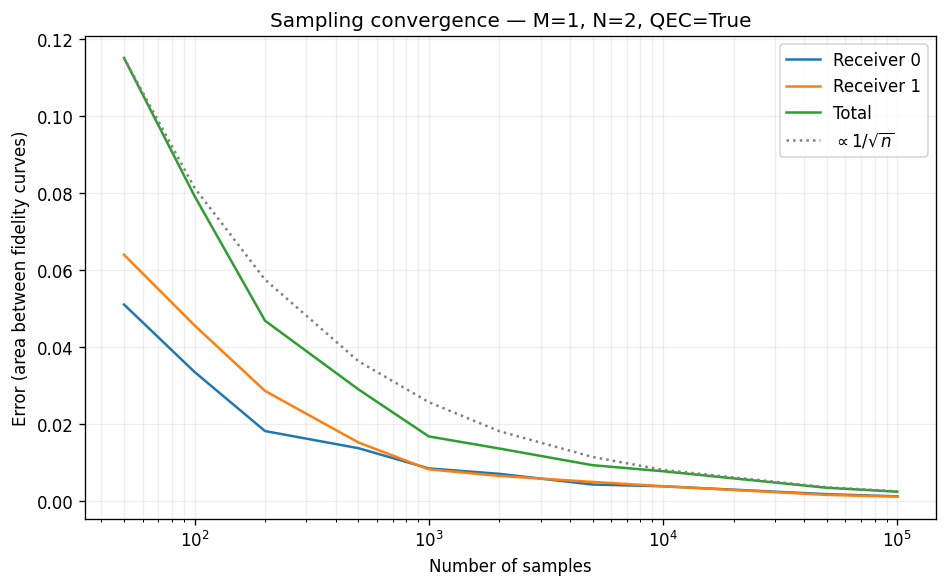
\includegraphics[width=1.05\linewidth]{mc_sampling_convergence.png}
    \caption{Error defined as the area between the fidelity curves for $p \in [0,1]$ of the MC trajectory sampling and the exact density matrix method for the $M{=}1$, $N{=}2$ protocol with depolarizing noise. As the number of samples increases, the Monte Carlo estimates converge to the exact values, demonstrating the validity of the sampling approach for estimating protocol performance under noise.}
    \label{Sampling Error Convergence}
\end{figure}

For larger receiver counts the $4^{5N}$ scaling of the encoded density matrix becomes prohibitive, so we estimate the post-noise state by Monte Carlo sampling of the depolarizing channels as Pauli trajectories. We exploit the Kraus decomposition $\mathcal{D}_p(\rho) = \sum_{P\in\{I,X,Y,Z\}} q_P\, P\rho P$ with $q_I = 1-p$ and $q_X = q_Y = q_Z = p/3$, which lets us replace the mixed-state evolution by a pure-state random walk:
\begin{enumerate}
    \item Start each trajectory from the encoded pure state $\ket{\widetilde\Psi^{(M,N)}}$ (dimension $D$, but only $O(D)$ memory because the state stays a vector).
    \item For each of the $5N$ physical receiver qubits, draw a Pauli $P\in\{I,X,Y,Z\}$ with probabilities $\{1-p,p/3,p/3,p/3\}$ and apply it to the trajectory by single-axis tensor contraction.
    \item Apply ideal $[[5,1,3]]$ recovery and decoding to each block. Because the trajectory is pure, the syndrome distribution is concentrated on a single outcome and we project onto the most-likely syndrome branch
    \begin{align}
        \ket{\psi} \mapsto \frac{V_{\mathrm{Dec}}\, E_{s^\star}\, P_{\mathcal{C}}\, E_{s^\star}\,\ket{\psi}}{\sqrt{p_{s^\star}}},
    \end{align}
    where $s^\star = \arg\max_s p_s$ and $V_{\mathrm{Dec}}$ maps each $[[5,1,3]]$ block back to a single qubit, reducing the per-trajectory state to dimension $(N{+}1)^M \cdot 2^N$.
    \item Accumulate the empirical density matrix on the decoded space, $\hat\rho = \tfrac{1}{n_s}\sum_{s=1}^{n_s} \ket{\psi_s}\!\bra{\psi_s}$, after $n_s$ trajectories.
\end{enumerate}
The remaining protocol stages (sender phase gates, Fourier measurement, byproduct correction, and partial trace) are then applied to $\hat\rho$ exactly as in the density-matrix path. This works because all of these operations act either on the sender register or as Pauli-covariant unitaries on the receivers, and therefore commute with the linear average over trajectories.

Per-trajectory cost is dominated by the $O(D)$ Pauli applications and the per-block decoding, so the overall cost of the estimator is $O(n_s \cdot N \cdot D)$ in time and $O(D)$ in memory, an improvement over the $O(D^2)$ exact storage. Because trajectories are independent, the statistical fluctuation in each scalar observable (here the per-receiver fidelity) decays as $1/\sqrt{n_s}$, and we verify this scaling in Fig.~\ref{Sampling Error Convergence} by measuring the area between the sampled and exact fidelity curves $F(p)$ for the $M{=}1$, $N{=}2$ protocol with QEC. We use $n_s$ in the range $10^2$--$10^5$ and demonstrate rapid convergence to the complete density matrix method for large samples.
\\

\subsection{Qiskit}


We implement the broadcasting protocol as a dynamic quantum circuit using Qiskit \cite{javadi2024qiskit}. Dynamic circuits incorporate mid-circuit measurements and real-time classical feedforward, features that are essential for both the sender Fourier-basis measurement with byproduct correction and the QEC syndrome-extraction-and-correction cycle \cite{corcoles2021dynamic}.

While numerical simulations allow us to control the error probability directly through adjusting the depolarizing probability, real hardware is more constrained. There are two parameters that we use instead as a proxy for the channel noise, these are idle delay time $\tau$ and optimization level. Idle delay time is a continuous adjustable delay that we add to the circuit in place of channel noise where we use exposure to the idle hardware noise in place of depolarizing probability. Hardware noise profiles are more complex, heterogeneous and correlated than simple independent depolarizing noise and can be more detrimental to highly entangled states such as our initial resource state. In order to explore this we characterized a basic fidelity circuit, where a random state is initialized, then a delay is added, before the state is rotated by the same random initial angle to the $\ket{0}$ state and measured in the logical basis. This is repeated and the outcome distribution is used as the fidelity estimate. The other noise parameter used was the optimization level $\ell \in \{0,1,2,3\}$. When a circuit is transpiled into gate instructions for a particular quantum hardware there are a number of ways to optimize the circuit performance, such as through circuit layout arrangement, coupling map selection, entanglement routing and dynamical decoupling \cite{javadi2024qiskit}. The predefined levels range from no optimization to combinations of more intensive optimization techniques. In Fig.~\ref{QEC Fidelity} we compare the performance of our basic fidelity circuit across a range of parameters. We see that the noise-free case (plotted with QEC) has no dependence on idle delay time as expected, and more surprisingly we see the introduction of our QEC protocol destroys the fidelity even at short delay times and using optimization. This is a strong indicator of the limitations of current hardware to accurately implement encoding, mid-circuit syndrome measurements and conditional corrections. With and without optimization, the single qubit fidelity far exceeds the QEC implementation, with the optimization level providing a strong benefit for short delay times over the unoptimizated case.

\begin{figure}[t]
    \centering
    
\includegraphics[width=\linewidth]{figures/qec513_delay_sweep_idle.png}
    \caption{Implementation of the $[[5,1,3]]$ quantum error correction code for a single qubit subject to a delay time before decoding on IBM Kingston. The fidelity of the output state with respect to the input state is plotted as a function of the delay time, demonstrating insufficient hardware performance to achieve a fidelity improvement over the unencoded case for any delay time.}
    \label{QEC Fidelity}
\end{figure}


When QEC is enabled, each receiver qubit is replaced by a five-qubit $[[5,1,3]]$ block using the encoding tensor $E_{b_1 b_2 b_3 b_4 b_5, q}$, defined by $E[\ldots,0] = \ket{0_L}$ and $E[\ldots,1] = \ket{1_L}$.

A schematic of the Qiskit circuit for the $M{=}1$, $N{=}2$ protocol without QEC is shown in Fig.~\ref{fig:circuit}. The circuit is built in six stages:

\begin{enumerate}
\item \textbf{State preparation.} The resource state $\ket{\Psi^{(M,N)}}$ (or its QEC-encoded variant) is loaded onto the sender register $\mathbf{a}$ ($M\cdot n_q$ qubits) and receiver register $\mathbf{r}$ ($N$ or $5N$ qubits).

\item \textbf{Delay.} A parametric delay $\tau$ is inserted on every receiver qubit. By sweeping $\tau$ we probe the effect of idle decoherence on the hardware.

\item \textbf{QEC recovery} (if enabled). Syndrome extraction and decoding are applied to each $[[5,1,3]]$ block reducing $5N$ physical qubits to $N$ decoded logical qubits.

\item \textbf{Sender phase gates.} Each sender~$j$ receives the diagonal unitary
\begin{align}
U_{a_j}(\theta_j) = \mathrm{diag}\!\left(e^{i(2k-N)\theta_j}\right)_{k=0}^{2^{n_q}-1},
\end{align}
which acts as a $2^{n_q}\times 2^{n_q}$ matrix with the phases $e^{i(2k-N)\theta_j}$ on the first $N{+}1$ diagonal entries and ones elsewhere.

\item \textbf{Fourier measurement.} Each sender's $n_q$-qubit register is rotated by $F_d^\dagger$, the inverse DFT on $d = N{+}1$ levels, embedded in a $2^{n_q}$-dimensional unitary:
\begin{align}
F_d[n,k] = \frac{\omega^{nk}}{\sqrt{d}},\qquad \omega = e^{2\pi i/d},
\end{align}
followed by a computational-basis measurement. This is equivalent to measuring in the Fourier basis $\{\ket{u_n}\}$.

\item \textbf{Classical feedforward.} For each possible $M$-tuple of sender outcomes $\bar{n}\in\{0,\dots,N\}^M$, the circuit conditionally applies a phase gate $P(-\phi)$ to every receiver qubit~\cite{corcoles2021dynamic}, where
\begin{align}
\phi = \frac{2\pi}{N+1}\!\left(\sum_{j=1}^{M} n_j \bmod (N{+}1)\right).
\end{align}

\end{enumerate}

\begin{figure*}
    \centering
    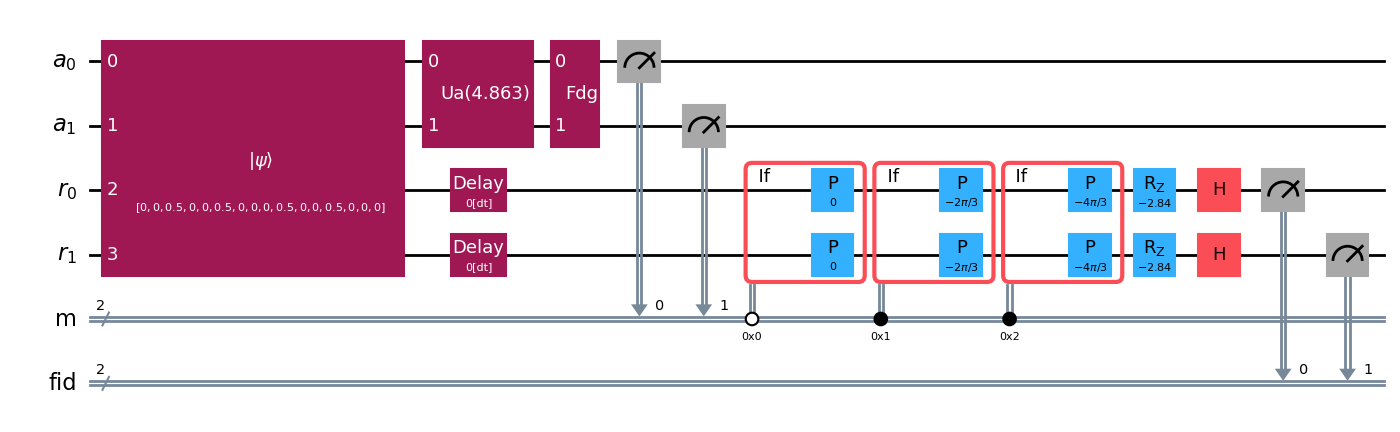
\includegraphics[width=0.95\linewidth]{m1n2qec0_circ.png}
    \caption{Qiskit circuit for the $M{=}1$, $N{=}2$ broadcasting protocol without QEC encoding. The sender qudit ($a_0, a_1$; two qubits encoding a qutrit) is initialized together with two receiver qubits ($r_0, r_1$) in the resource state $\ket{\Psi^{(1,2)}}$. After a parametric delay $\tau$, the sender phase gate $U_a(\theta)$ and inverse-DFT rotation $F_d^\dagger$ are applied, followed by a computational-basis measurement. Three conditional blocks (one per measurement outcome $n\in\{0,1,2\}$) each apply the corresponding phase correction $P(-2\pi n/3)$ to both receivers. Finally, $R_z(-\phi)$ and Hadamard gates rotate each receiver into the fidelity-measurement basis, and the outcomes are recorded.}
    \label{fig:circuit}
\end{figure*}

The $[[5,1,3]]$ error correction is implemented in the circuit using four shared ancilla qubits and Qiskit's dynamic-circuit primitives. For each five-qubit block the circuit appends three stages, illustrated schematically in Fig.~\ref{fig:circuit}.

Each of the four stabilizer generators $g_r\in\{XZZXI, IXZZX, XIXZZ, ZXIXZ\}$ is measured using one ancilla qubit. For each Pauli factor $P_i$ in the generator acting on block qubit~$i$:
\begin{itemize}
\item If $P_i = X$: apply $H$ to qubit~$i$, then $\mathrm{CX}(i,\mathrm{anc})$, then $H$ again.
\item If $P_i = Y$: apply $S^\dagger$ and $H$ to qubit~$i$, then $\mathrm{CX}(i,\mathrm{anc})$, then $H$ and $S$.
\item If $P_i = Z$: apply $\mathrm{CX}(i,\mathrm{anc})$ directly.
\item If $P_i = I$: no gate.
\end{itemize}
The ancilla is then measured, yielding syndrome bit $s_r$. Ancilla qubits are reset before each stabilizer measurement and reused across blocks.

The four syndrome bits $s = (s_1, s_2, s_3, s_4)$ form a 4-bit integer where a precomputed lookup table maps each of the 16 possible syndrome values to the corresponding single-qubit Pauli correction (or identity for $s=0$). The appropriate Pauli gate ($X$, $Y$, or $Z$) is conditionally applied to the identified qubit. All 15 single-qubit Pauli errors on the five physical qubits produce distinct nonzero syndromes, guaranteeing correction of any weight-1 error~\cite{laflamme1996perfect,gottesman1997stabilizer}.

The decoding unitary $V_{\Enc}^\dagger$ is constructed as a $32\times 32$ matrix via Gram--Schmidt orthogonalization \cite{nielsen2010quantum}. The first two columns of the encoding matrix $W$ are the normalized logical basis vectors $\ket{0_L}$ and $\ket{1_L}$; the remaining 30 columns are filled from the standard basis to complete an orthonormal set. Then $V_{\Enc}^\dagger = W^\dagger$ maps
\begin{align}
V_{\Enc}^\dagger \ket{0_L} &= \ket{00000}, &
V_{\Enc}^\dagger \ket{1_L} &= \ket{00001},
\end{align}
so the decoded logical qubit resides on the first physical qubit of each block.

The target output state for each receiver in the broadcasting protocol with $\alpha=\beta=1/\sqrt{2}$ lies on the equator of the Bloch sphere (the $XY$ plane):
\begin{align}
\ket{\psi_{\mathrm{target}}} = \frac{1}{\sqrt{2}}\!\left(e^{i\Phi}\ket{0} + e^{-i\Phi}\ket{1}\right),
\end{align}
where $\Phi = \sum_{j=1}^{M}\theta_j$ is the total sender angle.

We estimate the fidelity $F = \bra{\psi_{\mathrm{target}}}\rho_{\mathrm{out}}\ket{\psi_{\mathrm{target}}}$ using a single measurement basis per receiver qubit. The procedure appends two gates to each receiver qubit:
\begin{enumerate}
\item An $R_z(-\phi)$ rotation with $\phi = -2\Phi \bmod 2\pi$, which aligns the target state with $\ket{+}$:
\begin{align}
R_z(-\phi)\ket{\psi_{\mathrm{target}}} = \frac{1}{\sqrt{2}}\!\left(\ket{0} + \ket{1}\right) = \ket{+}.
\end{align}
\item A Hadamard gate $H$, which maps $\ket{+}\to\ket{0}$:
\begin{align}
H\,R_z(-\phi)\ket{\psi_{\mathrm{target}}} = \ket{0}.
\end{align}
\end{enumerate}
A computational-basis measurement is then performed. The probability of obtaining outcome~$0$ equals the fidelity:
\begin{align}
P(\text{outcome}=0) &= \bra{0}H\,R_z(-\phi)\,\rho_{\mathrm{out}}\,R_z(-\phi)^\dagger H^\dagger\ket{0} \nonumber \\
&= \bra{\psi_{\mathrm{target}}}\rho_{\mathrm{out}}\ket{\psi_{\mathrm{target}}} = F.
\end{align}
The fidelity measurements are stored in a separate classical register from the sender measurement outcomes, allowing both to be extracted from a single circuit execution. This approach requires only a single shot-statistics estimate per receiver qubit, making it efficient for hardware experiments where measurement overhead is a primary cost.
%\end{region}

\section{Results}
%\begin{region}

\begin{figure}[t]
    \centering
    
\includegraphics[width=\linewidth]{qec vs no qec vs sampling.png}
    \caption{Average receiver fidelity as a function of depolarizing probability $p$ for the $M{=}1$, $N{=}2$ protocol with and without $[[5,1,3]]$ quantum error correction compared against Monte Carlo trajectory sampling estimates. A zoomed view of the crossover region is included showing the range $p\in[0.130,0.145]$ where the $[[5,1,3]]$ protocol loses its advantage..}
    \label{qec_crossover}
\end{figure}

\begin{figure}[t]
    \centering
    
\includegraphics[width=\linewidth]{delay time vs fidelity 121 opt3.png}
    \caption{Fidelity of the output state with respect to the input state as a function of delay time on IBM Kingston, with $10,000$ shots per data point for the $M{=}1$, $N{=}2$ protocol without $[[5,1,3]]$ quantum error correction.}
    \label{qiskit_delay}
\end{figure}

We first verify the correctness of the exact density matrix and Monte Carlo sampling implementations by comparing their fidelity estimates for the $M{=}1$, $N{=}2$ protocol with QEC across a range of depolarizing probabilities $p$. As shown in Fig.~\ref{qec_crossover}, the two methods produce consistent results, with the sampling estimates converging to the exact curve as the number of trajectories increases. The plot also includes a zoomed view of the crossover region where the QEC-enhanced protocol loses its advantage over the unencoded case, which occurs around $p \approx 0.13$--$0.15$. This crossover point is higher than the rough estimate of $p \approx 0.1$ derived from the failure probability of the $[[5,1,3]]$ code, indicating that the effective noise after correction is less severe than the naive binomial approximation suggests. The exact density matrix method is used as the ground truth for benchmarking the sampling estimator, and the agreement between the two validates the use of Monte Carlo sampling for estimating protocol performance under noise, especially for larger receiver counts where the exact method becomes computationally infeasible. \\
%

We then implement the protocol on IBM quantum hardware using Qiskit, as described in the Methods section. Fig.~\ref{qiskit_delay} shows the fidelity of the output state with respect to the input state as a function of delay time $\tau$ for the $M{=}1$, $N{=}2$ protocol without QEC. The results indicate that the fidelity decreases with increasing delay time, which is expected due to decoherence effects on the hardware. However, even at short delay times, the fidelity is significantly below 1, suggesting that other sources of noise and imperfections in the hardware such as imperfect gate fidelity and readout error are also contributing to the degradation of the output state. This highlights the challenges of implementing quantum protocols on current noisy intermediate-scale quantum (NISQ) devices and underscores the importance of error mitigation and correction techniques for improving performance. Additionally, "spikes" of low fidelity are observed at certain delay times, which may be due to specific noise patterns or fluctuations in the hardware performance. Similar structures have been observed in other experiments and are referred to as "drop-outs" \cite{niu2024multi}. These quasi-periodic structures are suspected to arise due to the staggered dynamical decoupling regime implemented on idle qubits. Additionally, the protocol should be symmetric between receivers however in Fig.~\ref{qiskit_delay} we see clear and persistent differences in fidelity between Receiver 1 and Receiver 2. A possible cause of this could be the heterogeneity of coherence times between qubits, which for this particular device the T1 time ranges from $10.11-434.27\mathrm{\mu s}$\cite{javadi2024qiskit}.  \\
%

Lastly, we explore the feasibility of this protocol as the number of receivers scales. Our earlier analysis of independent depolarizing channels being the dominant source of decoherence breaks down as we increase the protocol size. This is demonstrated by the rapidly decreasing average receiver fidelity at $\tau=0$ for $M=1$. Independent channels should not be affected by the number of receivers, so the results we see in Fig.~\ref{protocol_scale} likely indicate correlated noise structures and the fragility of the shared entanglement resource state for larger protocol sizes. This is a significant challenge to the feasibility of this protocol for many practical use cases, indicating that hardware improvements and sophisticated QEC protocols are likely needed.


\begin{figure}
    \centering
    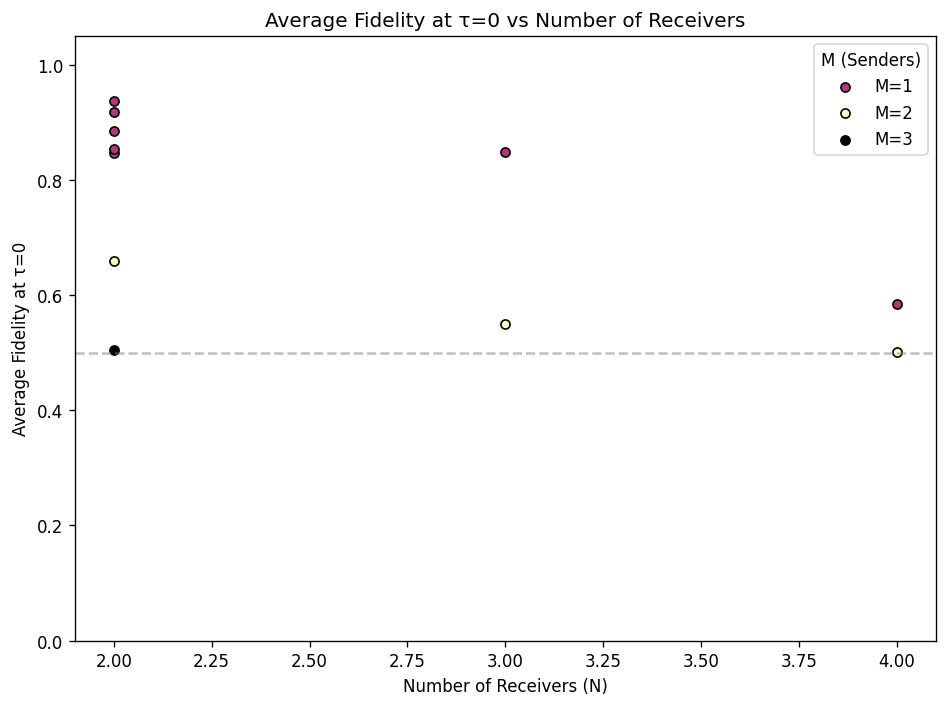
\includegraphics[width=\linewidth]{fidelity scaling hardware.png}
    \caption{The average receiver fidelity at $\tau=0$ for the $M$-sender, $N$-receiver protocol for a range of $M,N$ values, implemented on IBM Kingston with $10,000$ shots per data point.}
    \label{protocol_scale}
\end{figure}

%\end{region}

\section{Conclusion}
%\begin{region}
We have taken an existing quantum broadcasting protocol and studied its behavior under noise using a range of numerical techniques. We have then extended this protocol to include QEC with which we have demonstrated the region for with QEC is advantageous. Lastly, we have implemented this protocol on hardware, where we have analyzed the impact of QEC and found that current hardware used was not able to implement QEC advantageously. Our hardware results also indicate significant scaling challenges of this broadcasting protocol to larger network sizes. Most surprisingly, our hardware idle time results revealed a quasi-periodic "drop-out" phenomenon, that has been observed before but is not widely understood.
%

While broadcasting of quantum states using shared prior entanglement is a useful cryptographic primitive for distributed quantum computing and quantum networking our results indicate significant challenges in current implementation. On the experimental side, hardware idle noise demonstrates correlated noise structures that make large multipartite entangled states too fragile to scale effectively. Additionally, readout and gate fidelities are too low for basic QEC implementation to be effective. On the theory side, optimized broadcasting protocols are needed that incorporate natively tailored QEC techniques and are robust against correlated noise.

%\end{region}

\section{Acknowledgements}
%\begin{region}
This research was supported, in part, by a grant of computer time from the City University of New York High Performance Computing Center under NSF Grants CNS-0855217, CNS-0958379 and ACI-1126113. The code developed for this work is available at \color{red}Zenodo XXXXXXX. \color{black}Additionally we are grateful for the feedback and advice of IBM's Dr. Olivia Lanes and Dr. Nick Bronn regarding our fidelity results.
%\end{region}

\bibliography{apssamp}

\end{document}
%
% ****** End of file apstemplate.tex ******

